\chapter{Diagnosis}
\label{chap:diagnosis}

\section{The Company}
\label{sec:diagnosis-company}

This project will be conducted within a company called Highlander Computing Solution (HCS). The company provides business process services (e.g., customisation, deployment and support) for different clients using the same cloud ERP system (NetSuite) but with different business processes and organisational structures. HCS and their clients do not use any other BPM system although other systems are employed by HCS and clients as part of different business processes.\par

Currently, HCS provides basic customized NetSuite for their customers (currently eight - 8) based on different business process demands and business process automation. For example, HCS provides a service to generate support tickets automatically from customers’ emails. There is lots of space for modifying NetSuite. NetSuite allows users to reconfigure and customize their dashboards around the tasks and information they use most frequently. For example, we created customized Web pages and customized API points on NetSuite. It will provide you with the ability to extract and modify data in NetSuite using an external server. HCS provides a weekly report which extracts data from NetSuite for weekly technical support team meetings. It provides information about how many support tickets each employee solved. However, it only provides simple information, like the number of support tickets that have been raised and finished by each employee. Thus, we explored NetSuite configuration capabilities and customised API  for setting up our existing dashboard. \par

\section{The NetSuite System}

NetSuite ERP is an enterprise resource planning (ERP) system that runs on a vendor’s cloud platform as opposed to an on-premises network, allowing organizations to access the system through the Internet. NetSuite ERP is a SaaS system, which includes ERP, CRM, PSA, HR and Business Intelligence(BI) built on the NetSuite cloud platform which can be accessed over the Web. \par

From a customer perspective, clients can see the same views as HCS, but the majority of clients do not create workflows and scripts. HCS creates workflows and scripts for them.
Workflows can be created using XML called SuiteFlow in NetSuite, or graphical interface (drag and drop). NetSuite provides a developer scheme using JavaScript. They provide their API. Developers can upload the code in NetSuite from the Webpage. Define the code name and scope (component). Components are available to be used in workflow tasks.\par


\begin{figure}[!htb]
    \centering 
    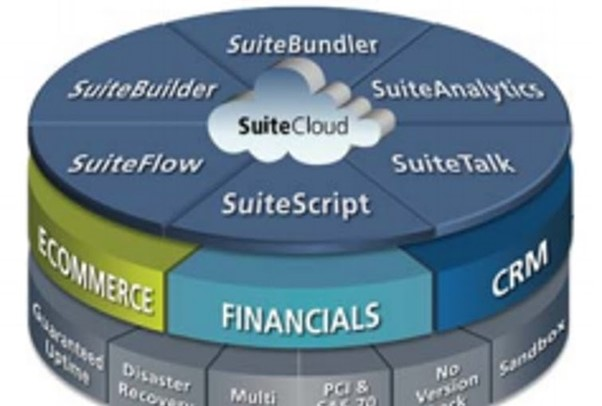
\includegraphics[scale=0.7]{resource/StructureOfSuiteCloud.jpg}
    \caption{The Structure Of SuiteCloud}
    \label{figure:structureSuiteCloud}
\end{figure}




There are five different ways to customise NetSuite based on Figure ~~\ref{figure:structureSuiteCloud}:
\begin{enumerate}
\item SuiteFlow  Figure ~\ref{figure:suiteFlow}
\item SuiteBuilder  Figure ~\ref{figure:suiteBuilder}
\item Suitetalk Figure ~\ref{figure:suiteTalk}
\item Suitescript Figure ~\ref{figure:suiteScript}
\item Suiteanalytics Figure ~\ref{figure:suiteAnalytics}
\end{enumerate}

Those will be described in the sequence.

\begin{figure}[!htb]
    \centering 
    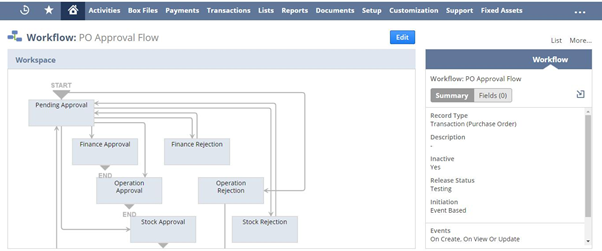
\includegraphics[scale=0.7]{resource/suiteFlow.png}
    \caption{The main view of the SuiteFlow component of NetSuite}
    \label{figure:suiteFlow}
\end{figure}

SuiteFlow is the way to customise business process automation by graphics ~\ref{figure:suiteFlow}. For example, HCS created a customized business process using SuiteFlow. NetSuite also provides an XML view for creating workflows.

\begin{figure}[!htb]
    \centering 
    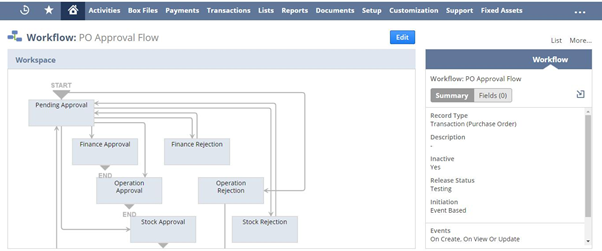
\includegraphics[scale=0.7]{resource/suiteFlow.png}
    \caption{Diagrams for SuiteBuilder}
    \label{figure:suiteBuilder}
\end{figure}


SuiteBuilder ~\ref{figure:suiteBuilder} is the way to bundle other customizations for installing into a test environment or production environment.

\begin{figure}[!htb]
    \centering 
    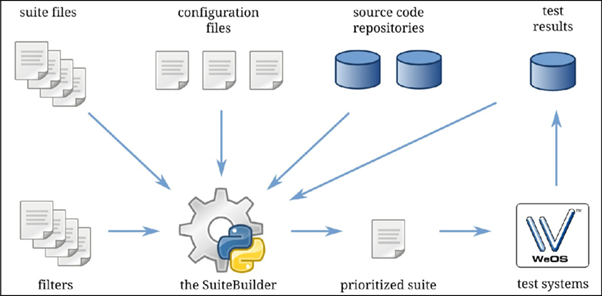
\includegraphics[scale=0.7]{resource/suiteTalk.png}
    \caption{SuiteTalk}
    \label{figure:suiteTalk}
\end{figure}

SuiteTalk ~\ref{figure:suiteTalk} is the NetSuite API (SOAP and REST ) for manipulating or extracting NetSuite data through API calls


\begin{figure}[!htb]
    \centering 
    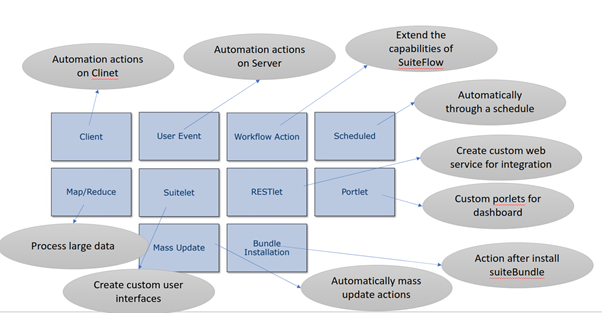
\includegraphics[scale=0.7]{resource/suitescript.png}
    \caption{Different Suitescript Functionality}
    \label{figure:suiteScript}
\end{figure}


SuiteScript ~\ref{figure:suiteScript} is the NetSuite platform built on JavaScript that enables complete customization and automation of business processes. Using the SuiteScript APIs, core business records and user information can be accessed and manipulated via scripts that are executed at pre-defined events. For example, field change, form submit, before reading, before write, or Web requests. They can also be scheduled to run at specific times.

In the sequence, we describe the main components of Suitescript ~\ref{figure:suiteScript}.

\begin{itemize}
    \item Suitelets Figure ~\ref{figure:suiteScript} — extensions to SuiteScript let you build a custom interface that is hosted within the NetSuite framework. Suitelets allow for completely custom HTML, Flash or NetSuite-based front-end development that can be built from scratch or by leveraging revolutionary SuiteScript UI Objects. Suitelets can also serve as the back-end for external HTML interfaces, providing complete flexibility in developing application extensions to NetSuite.
    \item SuiteScript UI Objects — Serve as extensions that let you build a custom interface that runs invisibly within the NetSuite framework.
    \item Portlet SuiteScript Figure ~\ref{figure:suiteScript} — scripted Dashboard portlets allow for listing of any NetSuite content on the Dashboard or inclusion of external data-feeds via RSS, HTML or Flash, as well as Web 2.0 mashups (e.g. instant messaging, maps, blogs, more) via embedded Inline HTML fields, or iFrames.
    \item Scheduled SuiteScript ~\ref{figure:suiteScript} — facilitates business process customization via JavaScript extensions and allows for records to be processed as a scheduled batch to automate workflows such as re-assignment of stale leads, drip-marketing or scheduling of collection calls based on days overdue.
    \item User Event SuiteScript ~\ref{figure:suiteScript} — SuiteScript can be used to enforce data validation and business rules. User Event SuiteScripts are triggered as users work with records and data changes in NetSuite as they open, edit or save records.
    \item Client SuiteScript ~\ref{figure:suiteScript} — field-level calculations, alerts and business logic are facilitated by SuiteScripts which run within the user's browser as they work with data and records within NetSuite. Additionally Server SuiteScript APIs can be invoked via the Client SuiteScript code to apply business logic beyond a single record.
\end{itemize}


SuiteAnalytics connect would help us to integrate with third-party applications to collect and analyze data. Used by both HCS and clients. HCS can build dashboards inside SuiteAnalytics


\begin{figure}[!htb]
    \centering 
    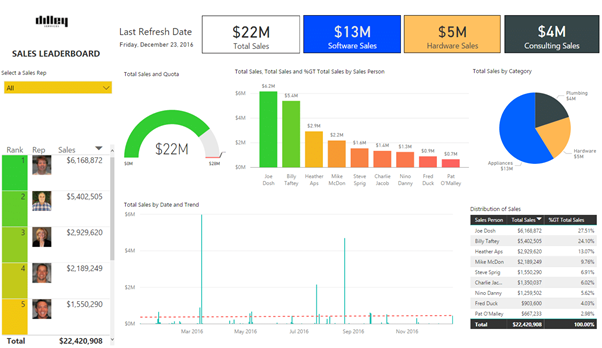
\includegraphics[scale=0.7]{resource/Suiteanalytics.png}
    \caption{One example from Suiteanalytics from NetSuite documentation}
    \label{figure:suiteAnalytics}
\end{figure}


NetSuite SuiteAnalytics provides real-time Saved Searches, Reporting, Key Performance Indicators (KPIs) Dashboard and Workbook features that are built into the NetSuite solution. Real-time transparency into company performance across all business functions—from summary level to transaction level. However, it doesn't reveal any business process details, such as Figure ~\ref{figure:monitor}.


\begin{figure}[!htb]
    \centering 
    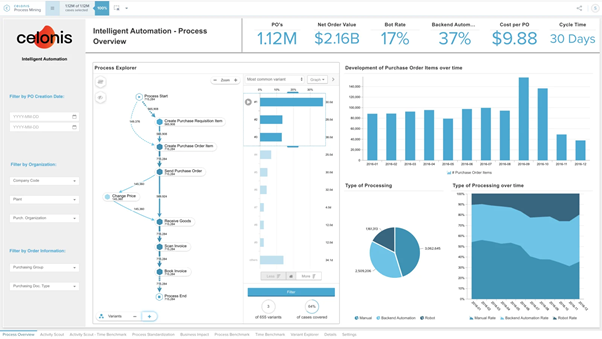
\includegraphics[scale=0.7]{resource/monitor.png}
    \caption{The example of Business process monitoring by Celonis}
    \label{figure:monitor}
\end{figure}








\section{Current practices of HCS with NetSuite}

HCS also provides an API server to communicate with NetSuite for integrating Microsoft graph API in Azure. HCS is deploying functionality only into NetSuite using SuiteBuilder ~\ref{figure:suiteBuilder}, however, it may upgrade to SuiteCloud or SuiteApp (NetSuite) in the future.

\begin{figure}[!htb]
    \centering 
    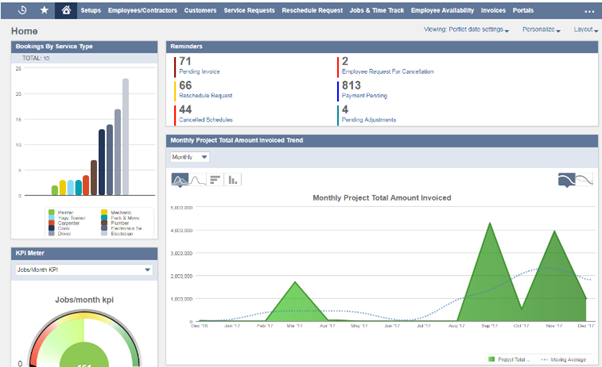
\includegraphics[scale=0.7]{resource/HCSNetSuite.png}
    \caption{The example of HCS monitoring}
    \label{figure:hcsMonitor}
\end{figure}


As part of HCS practices a dashboard is provided for weekly meetings.
Currently, HCS provides an external dashboard for weekly meetings. It provides some customized information, such as many weekly work tasks by supporting employees using SuiteAnalytics JDBC.

Currently, HCS provides an internal dashboard for weekly meetings. It provides some customized information, such as weekly work tasks by supporting employees using SuiteAnalytics.






\section{Problems faced by HCS}

There are eight customers in HCS at the moment. They are not in the same industry, six customers are in the manufacturing industry and the rest of them are in the service industry. HCS uses the NetSuite ERP system at moment, they are looking for selling the NetSuite and NetSuite application to customers. They provide different type of IT support services, at the same time, HCS provide support for eight NetSuite customers. 

We have identified a number of problems that will be the target of this study. The problems in the different industries at the moment, and we believe it is not connected to the category of the client. It may happen to any industry such as the financial department or support department. Different types of companies can only approach maximum efficiency and make key business process improvements when they understand how their workflows truly work. Humans alone can not perform this data extraction and analysis fast enough to make their organizations competitive. The problems from customers or HCS reveal that many deviations to the expected process model outcome happened at companies and caused the problems or potential problems.



\subsection{Problem 1}
Client 1 is in the manufacturing medical device industry. They have a manufacturing part of the process shown in figure 10. In this context, the “sales order" process involves three roles: sales team, manufacturing team and customer. A sales team is any user who faces customers and can raise sales orders and generate an estimate. A manufacturing team is composed of employees responsible for dealing with manufacturing, e.g. raise work order and pick components from stock. The system also includes customer roles, which are responsible for approving estimates of costs.

\begin{figure}[!htb]
    \centering 
    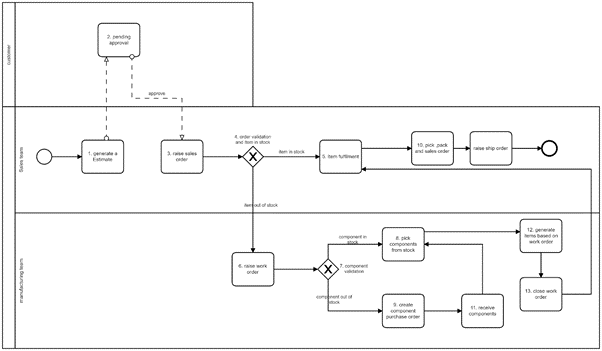
\includegraphics[scale=0.9]{resource/soAndwo.png}
    \caption{sales order and work order process}
    \label{figure:soAndwo}
\end{figure}

As shown in Figure ~\ref{figure:soAndwo}, the sales order process starts with:

\begin{itemize}
    \item the task “1. generate an estimate”, which is created by the “sales team”. The estimate needs to be approved by the customer (task "2. pending approval").
    \item Then, the approved estimate is converted into a  "sale order" (task "3. raise sale order"). A sale order can be  composed of several items. The process proceeds with a check for these items in stock (decision point "4. Order validation and item in stock").
    \item In case the items are in stock, they are picked up and packed (task "10. Pick, pack and sales order") before the order is fulfilled and the items shipped to the customer (task "raise ship order").
    \item Otherwise, a "Work order" for those items that are not in stock needs to be created by the "manufacturing team" (task "6. Raise work order").
    \item Once the "work order" is raised, the "manufacturing team" will check whether the components needed to assemble the items from the work order are available in stock (decision point "7. Component validation").
    \item If the components are in stock, the "manufacturing team" picks the components (task "8. Pick components from stock") and produce the items from the work order (task "12. Generate items based on work order").
    \item The work order is closed (task "13. Close work order") and the process continues from task "5. Item fulfilment". If a component is out of stock it needs to be purchased (task "9. Create component purchase order").
    \item Once the "manufacturing team" receives  the purchased components (task "11. Receive components"), the process continues from task "8. Pick components from stock".
\end{itemize}

This process has been reported to suffer from significant delays in shipping the items to customers. There are unpredictable risks in giving time estimates to customers, as there are two main points in the process that can cause delays:
\begin{enumerate}
    \item One problem faced by the client is estimation of delivery time by the sales team. Sometimes members of the sales team are new to the manufacturing industry, which makes it hard for them to give correct estimates. 
    However, this problem is compounded by the very nature of the manufacturing industry. Whenever an item is not available it needs to be assembled. 
    When the needed components are in stock, the assembly time can be reasonably calculated based on previous assembly of the same product. 
    However, when there is a need to purchase components the estimated time now depends on a third party. 
    
    \item Another problem faced by the client is dealing with live data. Not only is there a challenge in providing the customer with live data, but to update the data being used by the client in calculating their own estimates. For example, currently there is a shortage of components in the market due to supply chain issues, however, the client data is still out of data and not considering this fact.

\end{enumerate}

The client is looking for ways to understand what happens in the business in real-time or as soon as possible. Current monitoring capabilities only allow the identification of such problems later. 

Currently, four ways of monitoring at HCS:
\begin{enumerate}
    \item KPI monitoring (financial): look at reports at the end of month and compare the number of open orders with the expected value to be received and the actual value received.
    \item Report (operations): weekly/monthly reports. How many work orders opened in the period vs how many work orders are pending to finish vs how many work orders have been finished.
    \item Customer feedback: Customers complain when the order is late.
    \item "Save Search ": use SQL queries interface tools in NetSuite to dig out the data from NetSuite and analyse by customer support staff.
\end{enumerate}

Moreover, the client would like to use such data to calculate and compare expected process completion time with the actual time. 

To summarise, the proposed solution is that A dashboard for showing the times of the process. It starts with the average completion time of the whole process. It can then be broken down into average process times based on the "path". Then it can be broken down into average time per item per path.

\subsection{Problem 2}

Client 2 is in the computer and software service industry, they provide field service and another purchase order for their customer. In this context, there are two roles involved: sales team and field engineer team. A sales team is a team who is responsible to raise sales orders and purchase orders. A field service engineer team is an employee who provides IT support or product installation on site. 

\begin{figure}[!htb]
    \centering 
    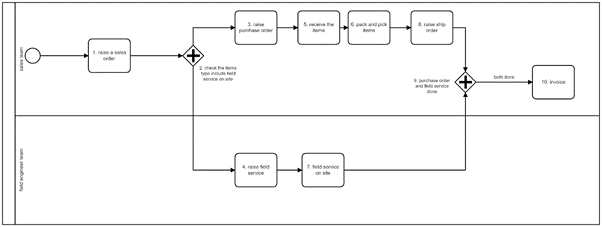
\includegraphics[scale=0.7]{resource/soAndFieldService.png}
    \caption{sales order and field service process}
    \label{figure:soAndfieldservice}
\end{figure}

As shown in Figure ~\ref{figure:soAndfieldservice}, the business process starts with:
\begin{enumerate}
    \item the task “1. raise a sales order”, which is created by the “sales team”. 
    \item Then, the process proceeds with a check for if these items' type are included "field service"(task "2). 
    \item in case those items' type include field service, field service team raise field service tickets(task "4. raise field service"). Then the field service team take an action on working on site(task "7 field service on site)
    \item otherwise, the sales team works on creating the purchase order(task "3. raise purchase order), after receiving the items(task "5. receive the item) from vendors.Additionally, the sales team is responsible to pack and ship the order(task "6. pack and pick items", task "8. raise ship order).
    \item subsequently, after ship order and field service are done, the sales team will be invoiced the transaction(task "10. invoice).
\end{enumerate}



Client 2  reports problems involving delayed sales orders. The delays have been caused by different reasons:
\begin{itemize}
\item the purchase order is delayed due to problems with the suppliers.
\item Field service work is delayed due to unforeseen circumstances.
\item There is a shortage of field engineers to perform the field work.
\end{itemize}

currently, HCS provides the monitor for explanation which sales order has been delayed by "save search", however, the monitor is difficult to explain why it has been delay, the lack of reasonable expected time for each business process are the one of the major problems for existing monitor. 

Moreover, the NetSuite provides full history logging about details of field engineers and their work allocation. At same time, the whole business process logging has been record in NetSuite.

In conclusion, the proposed solution is A dashboard for providing different reasons of delay the transaction process based on calculated reasonable process time. it also provides summarised historical information for senior executives to see where are the problems lie and why the problems happened. 

\subsection{Problem 3}

Client 3 is in the computer and software service industry, they provide support case service with the process shown on Figure ~\ref{figure:supportCase}.
\begin{figure}[!htb]
    \centering 
    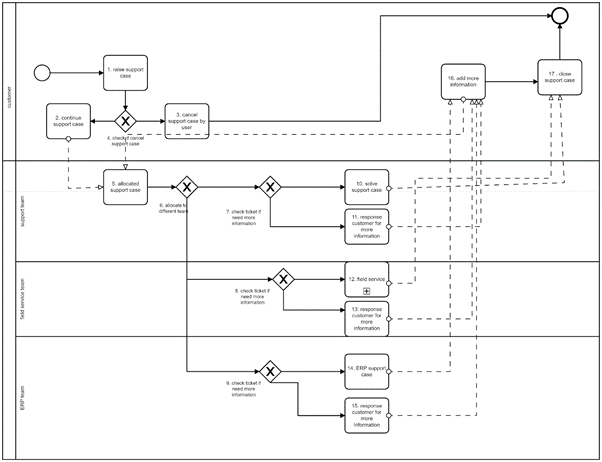
\includegraphics[scale=0.7]{resource/supportCase.png}
    \caption{support case process}
    \label{figure:supportCase}
\end{figure}

In this context, the “support case process” includes four different roles:
\begin{itemize}

\item A "customer" is the customers of Client 3 who is responsible to raise support cases.
\item The system also includes "support teams", which comprises allocated support cases and solve general support cases.
\item A "field service team" is responsible for solving support cases on site.
\item An "ERP team" is any user who focuses on support cases relevant to the NetSuite ERP system.
\end{itemize}

As Figre ~\ref{figure:supportCase} shown, the support case process starts with the task “1. raise support case” by customers, then there is an option for customers if they decide to cancel their support case (task "3. Cancel support case by user"). Support cases are allocated by a member of the "support team", which can decide to allocate it to any of the available teams based on the information included in the support case(task "6. allocate to different team ). There are three different situations based on different types of problems. Firstly, the support team may solve the problems by phone call or emails by themselves(task "10. slove support case"). Another, if there are required on-site helpdesk or service, the support team will transfer the support case to the field service team(task "12. field service"). Finally, if the support case is relevant to the ERP system, the support team will transfer the support case to the ERP team(task "14. ERP support case").

\begin{figure}[!htb]
    \centering 
    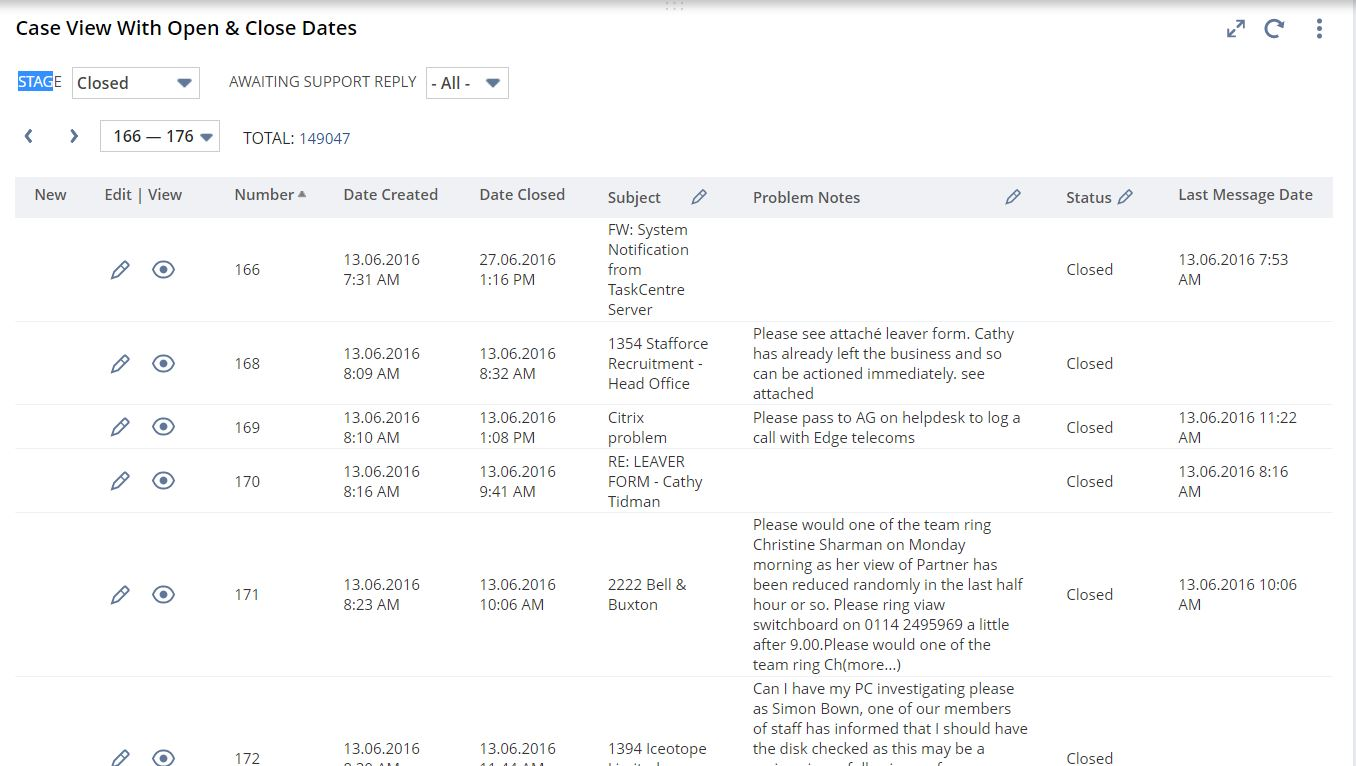
\includegraphics[scale=0.5]{resource/supportcaseHCS.JPG}
    \caption{support case existing dashboard}
    \label{figure:supportCaseHCS}
\end{figure}


Currently, there are dashboards to present the list of support cases which includes "latest message time" and "created time" like Figure ~\ref{figure:supportCaseHCS}. it only shows limited details such as the basic time stamp. However, the senior executives would like to know if there are some "spaghetti processes"(long and unmeaningful processes) or any other reasons. For example, it is because we are lacking in field engineering to solve the support case which delays the support case, and a support case has been delivered to different teams multiple times.

Predominantly, the proposed solution is a dashboard for showing the times  and conformance checking of the process to analysis and present the problems of business processes.it will consider about time perspective which focuses on the timing and frequency of events.Also, organisational perspective which focuses on information about resources hidden in the log, i.e., which actors (like,people, roles) are involved and how are they related.


\section{Final considerations} 

Clearly, there are three problems being presented, the proposed solution is a dashboard for showing the business processes from time and organisational perspectives.

For further study, predictive business monitoring is one of the future topics from time perspective. the business value monitoring is from the business values perspective, such as integrity, perseverance, determination.

Based on existing problems and proposed solutions, the next steps will provide ProM and Apromore to analyse the problems and design problems solutions.